\documentclass[12pt]{article}
\usepackage[a4paper, margin=.30in]{geometry}
%\usepackage{array}
\usepackage{fancybox}

\usepackage{graphicx, subfig, wrapfig, makecell,multirow }
\newcommand\headerMe[2]{\noindent{}#1\hfill#2}
\renewcommand \thesection{\Roman{section}}

\newcolumntype{M}[1]{>{\raggedright}m{#1}}

\usepackage{tikz}


\begin{document}

\headerMe{Royaume du Maroc}{année scolaire \emph{2024-2025}}\\
\headerMe{Ministère de l'Éducation nationale, }{  Professeur :\emph{Zakaria Haouzan}}\\
\headerMe{du Préscolaire et des Sports}{Établissement : \emph{Lycée SKHOR qualifiant}}\\

\begin{center}
Devoir surveillé N°1 \\
Durée 2h00\\
\underline{2-BAC Section des sciences expérimentales: Option de sciences physiques}\\

    \vspace{.2cm}
\hrulefill
\Large{Fiche Pédagogique}
\hrulefill\\
\end{center}
%end Headerss------------------------


%__________________Chimie ______________________-
%%%%%%%+_+_+_+_+_+_+_+_+_Partie1
\section[A]{Introduction }
\hspace{0.5cm}Le programme d'études de la matière physique chimie vise à croître un ensemble de compétences visant à développer la personnalité de l'apprenant. Ces compétences peuvent être classées en Compétences transversales communes et Compétences qualitatives associées aux différentes parties du programme.
\section{cadre de référence }
 \hspace{0.5cm}L'épreuve a été réalisée en adoptant des modes proches à des situations d'apprentissages et des situations problèmes, qui permettent de compléter les connaissances et les compétences contenues dans les instructions pédagogiques et dans le programme de la matière physique chimie et aussi dans le cadre de référence de l'examen national. 
 \\Tout en respectant les rapports d'importance précisés dans les tableaux suivants :
 \begin{center}
\begin{tabular}{|c||c||c|}
\hline
    \textbf{Restitution des Connaissances} & \textbf{Application des Connaissances} & \textbf{Situation Problème }\\
    \hline 
    $50\%$ & $25\%$ & $25\%$\\
    \hline
\end{tabular} 
\end{center}

\section{tableau de spécification}
 \begin{center}
\begin{tabular}{||c|c||c|c|c|c|}
\hline
     \multicolumn{2}{||c||}{\bf{   \hfill  Niveau d'habileté  \hfill } }
	& \makecell{Restitution \\des Connaissances} &\makecell{Application \\des Connaissances} & \makecell{Situation Problème} & la somme \\\hline

	%  
\multirow{1}{*}{ Les Ondes 53\%}
	& \makecell{Les Ondes\\mécaniques\\progressives}  & \makecell{6,5\%\\1Q - 0,5pts}  &\makecell{3,25\%\\1Q - 1pt} & \makecell{3,25\%\\} & 

	\multirow{3}{*}{\makecell{53\%\\13pts\\14Q\\65min}}\\\cline{2-5}
& \makecell{Les Ondes \\périodiques}  & \makecell{10\%\\1Q - 0,5pts}  &\makecell{5\%\\1Q - 1pt } & \makecell{5\%\\2Q - 1pt} &\\\cline{2-5}

& \makecell{Les Ondes \\lumineuse}  & \makecell{10\%\\4Q - 3pts}  &\makecell{5\%\\5Q - 4pt } & \makecell{5\%\\1Q - 2pt} &\\\hline

\multirow{2}{*}{ \makecell{Les\\Transformations\\d'un\\système\\chimique 47\%}}

& \makecell{lentes\\et\\rapides}  & \makecell{\\4\%\\3Q - 2.5pts}  &\makecell{2\% } & \makecell{1\%} &

\multirow{1}{*}{\makecell{47\%\\7pts\\12Q\\55min }}\\\cline{2-5}

& \makecell{Suivi\\temporel}  & \makecell{\\20\%\\1Q - 0,5pts}  &\makecell{\\10\%\\1Q - 0,5pts } & \makecell{\\10\%\\2Q - 1,25pts} &\\\hline



     \multicolumn{2}{||c||}{\bf{   \hfill  --  \hfill } }
& \makecell{50\%\\13Q - 11pts}  &\makecell{25\%\\6Q - 4,5pts } & \makecell{25\%\\8Q - 4,5pts} &\\\hline



\end{tabular} 
\end{center}

\newpage
\begin{center}
    \shadowbox{\bf{ Devoir surveillé $N^{\circ}$1 Semestre I} }
\end{center}
 \begin{center}

     \begin{tabular}{|c||c||c|}
    \hline
         \multicolumn{3}{||c||}{\bf{   \hfill  Chimie  \hfill (7pts)} }\\
         \hline
         \multicolumn{3}{||c||}{\bf{Suivi temporel d’une transformation chimique\dotfill} }\\
\hline
    \textbf{$N^{\circ}$Q. } & \textbf{Réponse } & \textbf{Note }\\
    \hline
    $1.$ &
         \makecell{les quantités de matière initiales des réactifs.\\
       $n_0(CaCO_{3(s)}) = 3.10^{-3} mol$ et $n_0(H_3O^+_{(aq)}) = 5.10^{-3}mol$
 }
    & $1pts$\\\hline
 %Q2
     $2.$ &
     \makecell{
		 le tableau d’avancement de cette réaction.\\
 \begin{tabular}{|c|c|c|c|c|c|c|}
    \hline
	\multicolumn{2}{|c|}{Equation de la réaction}& \multicolumn{5}{c|}{$2H_3O^+$ + $CaCO_3$ $\rightarrow$ $Ca^{2+}$ + $CO_2$ + $3H_2O$}\\\hline
    états  & avancement& \multicolumn{5}{|c|}{quantité de Matière en mol}\\\hline
    Etat initial          &    0        &  0,04&0,01&  0              &  0 & 0 \\\hline
   \makecell{Etat de \\transformation}&$x$ & $0,04-2x$ & $ 0,01-x$ & $x$  & $x$ & $x$ \\\hline
    Etat final&    $x_{max}$& $ 0,04 - 2x_{max}$ & $0,01 - x_{max}$ & $2x_{max}$  & $x_{max}$ & $x_{max}$ \\\hline
   % \cline{2-4}\
\end{tabular}\\
	 }
    & $0,5pts$\\\hline  
 %Q3
     $3$ &
       \makecell{ $x_{max} = 10^{-3}mol$ et le réactif limitant $H_3O^+$.}
    & $1pts$\\\hline  
 %Q4
     $4$ &
         \makecell{ Montrer que $V(CO_2) = 2,44.10^{-2}.x$}
    & $0.5pt$\\\hline  
 %Q5
     $5$ &
       \makecell{Montrer que $V(CO_2)_{t1/2} = 25mL $ et $t_{1/2} = 75s$}
    & $0,75pt$\\\hline  
	 $6$ &
       \makecell{la vitesse volumique de la réaction à l’instant de date t = 0 $V(t=0) = 0,24 mol/L.s$}
    & $0,5pts$\\\hline  

    $7$ &
	\makecell{La valeur du temps de
demi- réaction est inférieure à la valeur précédente }
    & $0,5pt$\\\hline  
     \multicolumn{3}{||c||}{\bf{Partie 2 : Mesure de conductivité \dotfill (2,25pts)} }\\
\hline
    \textbf{$N^{\circ}$Q } & \textbf{Réponse } & \textbf{Note }\\
    \hline
    $1$ &
         \makecell{ conductivité du mélange réactionnel à l’état initial.\\ $\sigma_i = \lambda_{H_3O^+}[H_3O^+] + \lambda_{Cl^-}[Cl^-] = 0,8526S/m$}
    & $0,75pt$\\\hline
 %Q2
 $2$ &
         \makecell{Montrer que l’avancement : $\sigma =-580.x(t) + \sigma_i$ }
    & $0,5pt$\\\hline
 %Q3
 $3$ &
         \makecell{Montrer que la vitesse volumique $v(t)= -17,2.\frac{d\sigma(t)}{dt}$ }
    & $1pt$\\\hline
      %Partie 2 : -----


%%Partie 2 : 
         %\multicolumn{3}{||c||}{\bf{Partie 2 : Suivi d’une transformation chimique\dotfill (2pts)}}\\
%\hline
%$1.$ &
         %\makecell{\\ % table dont forget 
             %\begin{tabular}{|c|c|c|c|c|c|}
    %\hline
    %\multicolumn{2}{|c|}{Equation de la réaction}& \multicolumn{4}{c|}{2CuO + C $\rightarrow$ 2Cu + $CO_2$}\\\hline
    %états  & avancement& \multicolumn{4}{|c|}{quantité de Matière en mol}\\\hline
    %Etat initial          &    0        &  12.38 &  1.4&  0              &  0 \\\hline
                 %\makecell{Etat de \\transformation}&    $x$      & $ 12.38 - 2x$ & $ 1.4 - x$ & $ 2x$  & $x$ \\\hline
    %Etat final            &    $x_{max}$& $ 12.38 - 2x_{max}$ & $1.4 - x_{max}$ & $2x_{max}$  & $x_{max}$ \\\hline
   %% \cline{2-4}\
%\end{tabular}
         %\\$\; $ }  
    %& $1pt$\\\hline
 %%Q2
   %$2$ &
         %\makecell{ l’avancement maximal $x_{max} = 1.4mol$ et le réactif limitant le carbone C(s) 
 %}
    %& $0.5pt$\\\hline  
 %%Q3
   %$3$ &
         %\makecell{ bilan de matière dans l’état final :\\ $n_f(CuO) = 9.58 mol$ et $n_f(C) = 0 mol$ et $n_f(Cu) = 2.8 mol$, $n_f(CO_2) = 1.4mol$ 
 %}
    %& $0.5pt$\\\hline  
%Physique : 
    %Partie 1 : 
\end{tabular} 
\end{center}

\begin{center}
  \begin{tabular}{|c||c||c|}
    \hline
         \multicolumn{3}{||c||}{\bf{   \hfill  Physique  \hfill (13pts)} }\\
         \hline
         \multicolumn{3}{||c||}{\bf{Partie 1 : le mouvement des vagues \dotfill (3pts)} }\\
\hline
    \textbf{$N^{\circ}$Q.} & \textbf{Réponse } & \textbf{Note }\\
    \hline
    $1$ &
         \makecell{
			 L’onde étudiée est transversale}
    & $0,5pt$\\\hline
 %Q2
 $2$ &
         \makecell{ la courbe représentant l’élongation du
point M. courbe 1}
    & $0,5pt$\\\hline
 %Q3
 $3$ &
         \makecell{
            Par exploitation des courbes précédentes, :\\
            $\tau = 8.10^{-2}s$ et $t_1 = 24.10^{-2}s$;\\
            $d = 26.10^{-2}m$ car $v = \frac{80.10^{-2}}{24.10^{-2}} = 3,33m/s$
      }
    & $2pt$\\\hline
 %Q3
 $3$ &
         \makecell{
           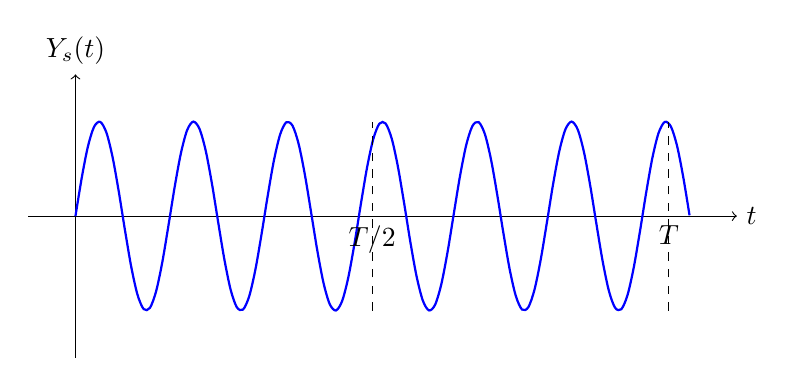
\begin{tikzpicture}[scale=1.2]
    \draw[->] (-0.5,0) -- (7,0) node[right] {\(t\)}; % Time axis
    \draw[->] (0,-1.5) -- (0,1.5) node[above] {\(Y_s(t)\)}; % Elongation axis
    % Sine wave
    \draw[thick,blue,domain=0:6.5,samples=100,smooth] 
        plot (\x,{sin(2*3.14159*\x r)});
    % Labels
    \node at (3.14,0) [below] {\(T/2\)};
    \node at (6.28,0) [below] {\(T\)};
    \draw[dashed] (3.14,-1) -- (3.14,1);
    \draw[dashed] (6.28,-1) -- (6.28,1);
\end{tikzpicture}
    }
    & $0,5pt$\\\hline
%1
 $1$ &
    \makecell{Montrer que $\lambda' = \sqrt{2}.\lambda$ }
    & $0,5pt$\\\hline

     \multicolumn{3}{||c||}{\bf{Partie 2 : Étude du phénomène ondulatoire.\dotfill (5pts)} }\\
\hline
%1
 $1$ &
 \makecell{Nom du phénomène observé diffraction la nature de
la lumière monochromatique }
    & $1pt$\\\hline
%2
 $2$ &
 \makecell{a l’aide de la figure 1 $\theta = \frac{L}{2.D}$ }
    & $0,5pt$\\\hline
 $3$ &
 \makecell{En utilisant les résultats des mesures $\theta = 3,15.10^{-3} rad$ }
    & $0,5pt$\\\hline

 $4$ &
 \makecell{la relation qui lie les grandeurs  $\theta = \frac{\lambda}{a}$ 
}
 
    & $0,5pt$\\\hline
 $5$ &
 \makecell{la valeur de la longueur d'onde  $\lambda = 0,63m$ \\elle appartient au domaine visible 
}
 & $0,5pt$\\\hline

 $6$ &
 \makecell{-on remplace la lumière émise par le LASER (lumière rouge) par une lumière bleue\\L diminue\\
	 -n diminue la largeur de la fente a L augmente\\
	 -différencier expérimentalement une lumière monochromatique d’une lumière \\ polychromatique  par un prisme
}
 & $2pt$\\\hline











  \end{tabular}
  \end{center}


\end{document}
